

\chapter{METODOLOGÍA} \label{chap:metodologia}

Este capítulo describe el procedimiento metodológico seguido para desarrollar e 
implementar los modelos de clasificación de retinopatía diabética basados en aprendizaje 
profundo. La metodología se estructura en cinco etapas principales: primero, 
la recopilación y caracterización de conjuntos de datos de imágenes de fondo de ojo; 
segundo, el preprocesamiento y balanceo de datos para optimizar la calidad del 
conjunto de entrenamiento; tercero, la selección de tecnologías y herramientas de 
desarrollo; cuarto, la configuración e implementación de las arquitecturas CNN con 
técnicas de regularización; y finalmente, la definición de métricas de evaluación para 
validar el desempeño de los modelos. La Figura~\ref{fig:metodologia-general} presenta un diagrama que sintetiza el flujo
completo del proceso metodológico implementado.

\begin{figure}[H]
	\centering
	\caption{Estructura metodológica propuesta para la clasificación de retinopatía 
diabética mediante aprendizaje profundo}
	\label{fig:metodologia-general}
	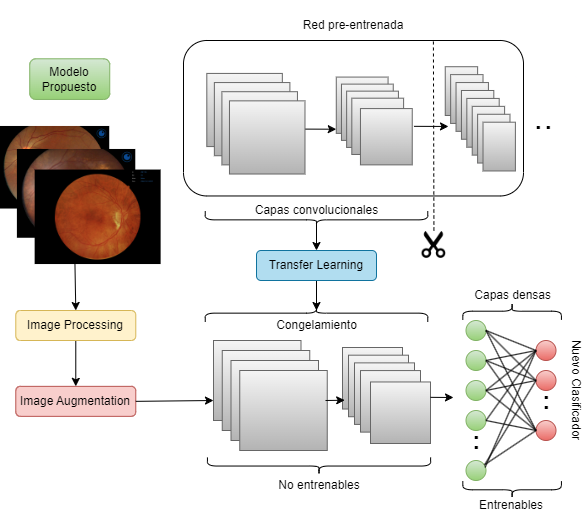
\includegraphics[width=1\textwidth]{imágenes/metodología/MODELO.png}
	\caption*{\textit{Fuente: Elaboración propia}}
\end{figure}

\section{CONJUNTOS DE DATOS} \label{sec:conjuntos-datos}

Una etapa clave en la construcción de una red neuronal convolucional (CNN) es la 
recopilación de datos, ya que el rendimiento del modelo depende en gran medida tanto de 
la calidad como de la diversidad del conjunto utilizado. Para que el entrenamiento sea 
efectivo, las imágenes deben reflejar con precisión las distintas condiciones del 
problema y pueden obtenerse a partir de repositorios públicos, fuentes en línea o 
mediante técnicas de generación artificial. Es esencial que cada imagen esté 
correctamente clasificada según corresponda, ya que una mala etiquetación puede afectar 
negativamente el aprendizaje del modelo. Por ello, es importante realizar una curaduría 
rigurosa del dataset, priorizando imágenes representativas y bien definidas.

En el desarrollo de este proyecto se utilizaron distintos conjuntos de datos para 
garantizar la robustez y generalización del modelo. Inicialmente se exploraron datasets 
disponibles en repositorios públicos, junto con un conjunto de datos de propiedad 
privada. La fase experimental inicial se llevó a cabo con el dataset de Kaggle debido a 
su gran volumen de imágenes. Posteriormente se utilizaron los datasets públicos
MESSIDOR-2, IDRiD y uno privado denominado FOSCAL para evaluar la capacidad de
generalización del modelo final mediante validación externa: el modelo, entrenado
exclusivamente con el dataset de Kaggle, fue evaluado directamente sobre estos tres
conjuntos sin reentrenamiento ni ajuste de pesos.

\subsection{Dataset de Kaggle (Entrenamiento)}

Es el dataset principal que se utilizó para entrenar y validar los modelos
experimentales. Cuenta con un amplio conjunto de datos compuesto por imágenes de retina
en alta resolución, obtenidas a partir del repositorio \textit{Diabetic Retinopathy
Detection 2015}, disponible en la plataforma Kaggle. Las imágenes provienen de EyePACS,
una red de telemedicina para tamizaje de retinopatía diabética que opera principalmente
en centros de atención primaria de California, Estados Unidos
\myfootcite{cuadros2009eyepacs}. Las imágenes fueron capturadas bajo
diversas condiciones y con distintos tipos de cámaras, lo que introduce variabilidad en
aspectos como la resolución, la iluminación y la orientación.

Cada registro corresponde a un paciente, identificándose ambos ojos mediante un nombre de 
archivo que incluye el número de paciente seguido de \enquote{izquierda} o
\enquote{derecha} (por 
ejemplo: \texttt{1\_izquierda.jpg}). Cada imagen fue evaluada por un especialista 
clínico, quien asignó un grado de severidad de retinopatía diabética utilizando una
escala ordinal de 0 a 4: 0, sin retinopatía diabética; 1, leve; 2, moderada; 3, severa;
y 4, retinopatía diabética proliferativa.

La naturaleza heterogénea del conjunto se evidencia en las diferencias anatómicas y de 
orientación presentes en las imágenes: algunas muestran la retina con una disposición 
convencional (mácula a la izquierda y nervio óptico a la derecha en el caso del ojo 
derecho), mientras que otras presentan una orientación invertida, similar a la observada 
a través de un microscopio durante un examen clínico. La orientación puede determinarse a 
partir de la posición relativa entre la mácula y el nervio óptico, así como por la 
presencia de muescas laterales en la imagen.

Es importante señalar que el conjunto contiene ruido, tanto en las imágenes (como 
artefactos, desenfoque, subexposición o sobreexposición), como en las etiquetas, debido a 
la subjetividad inherente a la evaluación clínica. Por esta razón, uno de los retos 
principales de este estudio es desarrollar algoritmos robustos, capaces de enfrentar 
dicha variabilidad y el ruido presente en los datos, asegurando un desempeño confiable en 
escenarios reales de aplicación.

\subsection{MESSIDOR-2 (Validación externa)}

Es una base de datos de imágenes de fondo de ojo diseñada para evaluar algoritmos de
detección de retinopatía diabética, particularmente para la clasificación de casos
referibles. Contiene un total de 1,748 imágenes correspondientes a 874 exámenes de
pacientes, provenientes de tres departamentos de oftalmología en Francia: el Hospital
Universitario de Brest, el Hospital Universitario de Saint-Étienne y el Hôpital
Lariboisière de París \myfootcite{decenciere2014messidor}. Las imágenes fueron
capturadas con cámaras no midriáticas Topcon TRC NW6, NW7 y Nidek AFC-210, con
un campo de visión de 45°. Las imágenes presentan resoluciones variables, típicamente
entre $1440 \times 960$ y $2304 \times 1536$ píxeles, y están centradas en la mácula.

Este conjunto cuenta con: etiquetas de gradación de retinopatía diabética (RD) en una 
escala de 0 a 3; etiquetas de edema macular, validadas por especialistas; y metadatos 
como el diámetro pupilar y la calidad técnica de cada imagen. Gracias a su calidad, 
volumen y amplia adopción en la comunidad científica, MESSIDOR-2 es ampliamente empleado 
como benchmark para evaluar el rendimiento y la generalización de modelos de 
clasificación de RD, especialmente en escenarios de validación externa y estudios 
comparativos.

\subsection{IDRiD (Validación externa)}

El \textit{Indian Diabetic Retinopathy Image Dataset} contiene un total de 516 imágenes 
de retina en alta resolución ($4288 \times 2848$ píxeles), capturadas con una cámara Kowa 
VX-10$\alpha$ con un campo de visión de 50\textdegree, centradas en la mácula. Las 
imágenes provienen de pacientes del Aravind Eye Hospital en India y están acompañadas de 
anotaciones detalladas realizadas por expertos clínicos.

Este conjunto incluye: etiquetas de clasificación de severidad de RD; segmentaciones a 
nivel de píxel para lesiones específicas como microaneurismas, hemorragias, exudados 
duros y blandos; y segmentaciones de estructuras anatómicas como la fóvea y el disco 
óptico. El dataset se divide en un conjunto de entrenamiento con 413 imágenes y un 
conjunto de prueba con 103 imágenes, lo que lo hace especialmente útil tanto para tareas 
de clasificación como de segmentación.

\subsection{FOSCAL (Validación externa)}

El dataset FOSCAL está compuesto por 1,538 imágenes de fondo de ojo, obtenidas gracias al 
Centro de Prevención y Consultoría en Glaucoma de Bucaramanga (Fundación Oftalmológica de 
Santander - FOSCAL). Las imágenes estaban acompañadas de un archivo plano que detalla las 
anomalías presentes, incluyendo el nivel de retinopatía diabética (RD), lo que permitió 
organizarlas con sus respectivas etiquetas.

El proceso de etiquetado fue realizado por especialistas médicos mediante una plataforma 
web diseñada específicamente para la lectura y tamizaje. Esta plataforma incluía 
funcionalidades para descartar imágenes de baja calidad o no evaluables, garantizando así 
la confiabilidad de los datos. Este dataset representa condiciones clínicas locales y fue 
utilizado como validación externa para evaluar el desempeño del modelo en un contexto 
colombiano específico.

\subsection{Distribución de datos}

La Tabla~\ref{tab:distribucion_clases} presenta la distribución de imágenes por clase de 
severidad en cada uno de los datasets utilizados, mostrando la variabilidad en la 
distribución de clases entre diferentes fuentes de datos.

\begin{table}[H]
	\centering
	\renewcommand{\arraystretch}{1.5}
	\caption{Distribución de imágenes por clase de severidad de retinopatía diabética 
en los distintos datasets}
	\label{tab:distribucion_clases}
	\begin{tabularx}{\textwidth}{X c c c c c c c}
		\hline
		\textbf{Dataset} & \textbf{No RD} & \textbf{Leve} & \textbf{Moderada} & 
\textbf{Severa} & \textbf{Prolif.} & \textbf{Total} & \textbf{Uso} \\
		\hline
		Kaggle & 25,810 & 2,443 & 5,292 & 873 & 703 & 35,121 & Entrenamiento \\
		MESSIDOR & 1,017 & 270 & 347 & 114 & --- & 1,748 & Validación ext. \\
		IDRiD & 213 & 117 & 54 & 56 & 76 & 516 & Validación ext. \\
		FOSCAL & 302 & 34 & 23 & 40 & 16 & 415 & Validación ext. \\
		\hline
	\end{tabularx}
	\caption*{\textit{Fuente: Elaboración propia}}
\end{table}

Como puede observarse en la Tabla~\ref{tab:distribucion_clases}, el desbalance hacia la
clase No RD no es exclusivo del dataset de Kaggle (73.5\%): FOSCAL presenta una
proporción similar (72.8\%), mientras que IDRiD resulta considerablemente más balanceado
(41.3\% de la clase mayoritaria). MESSIDOR, por su parte, no incluye casos etiquetados
como retinopatía proliferativa, lo que ilustra la heterogeneidad en los criterios de
recolección y etiquetado entre los datasets externos utilizados para la validación, un
factor que se retoma en la discusión de la capacidad de generalización del modelo
(Capítulo~\ref{chap:discusion}).

\subsection{División de datos para entrenamiento y validación} \label{subsec:division-datos}

El dataset de Kaggle se dividió en tres subconjuntos siguiendo una estrategia de
partición estratificada. Esta elección responde directamente al marcado desbalance de
clases del conjunto original, descrito en la Sección~\ref{subsec:balanceo-clases}, donde
la clase 0 (sin RD) representa aproximadamente el 73\% de las imágenes frente a apenas un
2\% de la clase 4 (RD proliferativa): una partición completamente aleatoria podría, por
azar, generar subconjuntos con proporciones de clase distintas entre sí —por ejemplo, un
conjunto de prueba con una proporción de casos severos notablemente distinta a la del
conjunto de entrenamiento—, lo que dificultaría comparar las métricas obtenidas entre
subconjuntos y podría sesgar la evaluación del modelo. La partición estratificada busca
mantener aproximadamente las mismas proporciones de clase en los tres subconjuntos,
haciendo la evaluación más comparable y confiable:

\begin{itemize}
    \item \textbf{Conjunto de entrenamiento (70\%):} 24,585 imágenes utilizadas para el 
ajuste de pesos del modelo.
    \item \textbf{Conjunto de validación (15\%):} 5,268 imágenes utilizadas para la 
optimización de hiperparámetros y detección de sobreajuste durante el entrenamiento.
    \item \textbf{Conjunto de prueba interno (15\%):} 5,268 imágenes reservadas para la 
evaluación final del modelo antes de validación externa.
\end{itemize}

Esta división se implementó utilizando la función \texttt{train\_test\_split} de
scikit-learn con el parámetro \texttt{stratify} para asegurar que la distribución de
clases se mantuviera consistente en todos los subconjuntos.

Es importante precisar el orden en que se ejecutan la partición y el balanceo de clases
(Sección~\ref{subsec:balanceo-clases}), ya que invertirlo puede introducir fuga de
datos (\textit{data leakage}): si el balanceo se aplicara antes de dividir el conjunto
—por ejemplo, duplicando imágenes de las clases minoritarias mediante sobremuestreo—,
copias de una misma imagen podrían terminar repartidas entre entrenamiento, validación y
prueba, de modo que el modelo sería evaluado, al menos parcialmente, con imágenes que ya
observó durante el entrenamiento. Para evitar este riesgo, la partición
estratificada descrita en esta sección se realiza siempre \textbf{primero}, sobre las
imágenes originales sin duplicar; el balanceo de clases (submuestreo o sobremuestreo,
según el escenario) se aplica \textbf{después}, y únicamente sobre el conjunto de
entrenamiento resultante. Los conjuntos de validación y prueba conservan la distribución
de clases real del dataset, sin balancear, de manera que las métricas reportadas
reflejan el desempeño del modelo sobre datos no vistos durante el entrenamiento y con una
proporción de clases representativa del problema original.

\section{PREPROCESAMIENTO DE LAS IMÁGENES} \label{sec:preprocesamiento}

Durante el análisis exhaustivo del conjunto de datos, se identificaron varios problemas 
que afectan negativamente el desempeño de los modelos. Entre los principales desafíos se 
encontraron una cantidad significativa de imágenes dañadas o de baja calidad, las cuales 
dificultan el proceso de aprendizaje del modelo, así como un notable desbalance entre las 
clases, especialmente por la predominancia de la clase correspondiente a pacientes sanos. 
Este desbalance puede llevar al modelo a sesgar sus predicciones hacia la clase 
mayoritaria, reduciendo su capacidad de generalización. Por ello fue necesario aplicar 
estrategias específicas de limpieza, filtrado y balanceo, orientadas a mejorar la calidad 
de los datos sin eliminar muestras valiosas ni conservar imágenes que pudieran perjudicar 
el entrenamiento.

\subsection{Depuración de imágenes defectuosas} \label{subsec:depuracion-imagenes}

Durante el proceso de exploración y limpieza del conjunto de datos, se identificó un 
número considerable de imágenes que presentaban problemas severos de iluminación: algunas 
eran casi completamente oscuras y otras excesivamente brillantes. En ambas situaciones 
resultaba imposible distinguir adecuadamente la circunferencia del globo ocular o las 
estructuras internas relevantes para la detección de retinopatía diabética. A pesar de 
ello, estas imágenes estaban etiquetadas con niveles de severidad entre 0 y 4, lo que 
indicaba que habían sido consideradas válidas en el conjunto original. No obstante, su 
falta de información visual útil no solo limita su valor diagnóstico, sino que también 
puede introducir ruido y dificultar el proceso de aprendizaje del modelo.

Para abordar este problema, se diseñó un procedimiento automático de limpieza basado en 
el análisis del brillo promedio de las imágenes. Esta estrategia consistió en convertir 
cada imagen a escala de grises y calcular su luminosidad media. Si el valor promedio se 
encontraba por debajo de un umbral establecido para imágenes demasiado oscuras 
($\mu_{brillo} < 10$) o por encima de un umbral para imágenes excesivamente brillantes 
($\mu_{brillo} > 245$), la imagen se consideraba no apta para el entrenamiento. Aquellas 
que cumplían con estos criterios eran automáticamente separadas del conjunto principal y 
movidas a una carpeta de exclusión. Este proceso se implementó utilizando OpenCV y NumPy 
en Python, y permitió filtrar de manera eficiente las imágenes que no aportan información 
significativa.

\subsection{Balanceo de clases} \label{subsec:balanceo-clases}

El conjunto de datos original presenta un marcado desbalance entre las clases, lo cual 
representa un desafío importante para la construcción de clasificadores. En particular, y 
en el escenario multiclase, la clase 0 (pacientes sanos) representa aproximadamente el 
73\% del total de muestras, mientras que la clase 4 (retinopatía diabética 
proliferativa), la forma más severa de la enfermedad, apenas alcanza el 2\%. Esta 
relación —muy superior a 4:1 en el caso multiclase— tiende a sesgar el aprendizaje hacia 
la clase mayoritaria y reduce la capacidad del modelo para detectar correctamente las 
clases menos representadas. Este efecto del desbalance en el rendimiento de 
clasificadores ha sido ampliamente documentado en la literatura sobre aprendizaje con 
datos desbalanceados \myfootcite{johnson2019survey} \myfootcite{mustapha2024class}.

En general, para mitigar los problemas derivados del desbalance, se aplicaron dos
estrategias principales: una reducción de la clase 0 mediante submuestreo (eliminando
aleatoriamente parte de sus imágenes hasta acercarla a las demás clases) y un aumento
artificial de las clases minoritarias mediante técnicas de aumento de datos (data
augmentation), es decir, la generación de nuevas muestras a partir de transformaciones
de las imágenes existentes, cuyos detalles se describen en la
Subsección~\ref{subsec:aumento-datos}. En el escenario multiclase, un muestreo aleatorio directo sobre la
clase 0 no resultó óptimo, ya que esta contenía un número considerable de imágenes con 
ruido o baja calidad. Para evitar descartar ejemplos útiles y conservar otros 
potencialmente perjudiciales, se realizó primero una limpieza manual, con lo que se 
obtuvo una base más depurada que facilitó el posterior balanceo entre las cinco 
categorías.

En el clasificador binario, en cambio, el enfoque consistió en agrupar todas las
categorías con retinopatía en una sola clase (RD) frente a las imágenes sin enfermedad
(No RD). Sobre el conjunto de entrenamiento resultante de la partición
(Sección~\ref{subsec:division-datos}) se aplicó sobremuestreo aleatorio
(\texttt{RandomOverSampler} de la librería \texttt{imbalanced-learn}), que duplica
imágenes de la clase minoritaria hasta lograr una proporción cercana al 50:50 entre
ambas clases; los conjuntos de validación y prueba no se balancean y conservan la
proporción real de clases. Aplicar el sobremuestreo después de la partición, y
solo sobre el conjunto de entrenamiento, evita que copias duplicadas de una misma imagen
terminen repartidas entre entrenamiento y evaluación.

\subsection{Aumento de datos} \label{subsec:aumento-datos}

El aumento de datos, aunque es una técnica común y poderosa dentro del aprendizaje 
profundo, debe ser aplicado con cautela, especialmente cuando se trabaja con modelos 
preentrenados. Estos modelos, al contar con una gran cantidad de parámetros ajustables, 
pueden ser más propensos al sobreajuste si se les expone a transformaciones que alteran 
excesivamente la naturaleza de los datos originales.

Para mitigar este riesgo, se priorizó el uso de transformaciones que introducen 
variabilidad sin modificar la estructura fundamental de la imagen. Estas técnicas 
preservan la integridad visual de las retinografías al tiempo que enriquecen la 
diversidad del conjunto de entrenamiento \myfootcite{shorten2019survey}. Se implementó un 
conjunto de transformaciones geométricas moderadas utilizando la clase 
\texttt{ImageDataGenerator} de Keras, que permitió generar nuevas muestras a partir de 
imágenes existentes de forma controlada. La Tabla~\ref{tab:data-augmentation} detalla las
seis transformaciones aplicadas y el rango o parámetro utilizado en cada una.

\begin{table}[H]
\centering
\renewcommand{\arraystretch}{1.3}
\caption{Configuración de transformaciones de aumento de datos aplicadas}
\label{tab:data-augmentation}
\begin{tabularx}{\textwidth}{l X c}
\hline
\textbf{Transformación} & \textbf{Descripción} & \textbf{Parámetro} \\ \hline
Rotación & Rotación aleatoria de la imagen & $\pm 10^\circ$ \\
Zoom & Acercamiento/alejamiento aleatorio & $\pm 5\%$ \\
Desplazamiento horizontal & Traslación horizontal de la imagen & $\pm 5\%$ \\
Desplazamiento vertical & Traslación vertical de la imagen & $\pm 5\%$ \\
Volteo horizontal & Reflexión horizontal (flip) & Probabilidad 0.5 \\
Modo de relleno & Interpolación para píxeles faltantes & Nearest \\ \hline
\end{tabularx}
\caption*{\textit{Fuente: Elaboración propia}}
\end{table}

Estas operaciones fueron aplicadas únicamente a las clases minoritarias (1, 2, 3, 4) con 
el objetivo de equilibrar la distribución del conjunto de datos. Al concluir los procesos 
de limpieza y aumento de datos, se obtuvo un conjunto de datos significativamente más 
robusto, con menos información que pudiera interferir con el aprendizaje del modelo. 
Además, se ha logrado un balance adecuado entre las clases, lo que favorece una mayor 
capacidad de generalización en el modelo. La Tabla~\ref{tab:clases_aumentadas} muestra la 
distribución final del dataset optimizado.

\begin{table}[H]
	\centering
	\renewcommand{\arraystretch}{1.5}
	\caption{Distribución de clases en el conjunto de datos aumentado y balanceado}
	\label{tab:clases_aumentadas}
	\begin{tabular}{c c c c}
		\hline
		\textbf{Nivel de RD} & \textbf{Etiqueta} & \textbf{Cantidad de Imágenes} 
& \textbf{Porcentaje (\%)} \\
		\hline
		0 & No RD & 7,000 & 23.33 \\
		1 & Leve & 6,998 & 23.33 \\
		2 & Moderada & 6,000 & 20.00 \\
		3 & Severa & 4,996 & 16.65 \\
		4 & Proliferativa & 4,999 & 16.66 \\
		\hline
		\textbf{Total} & & \textbf{29,993} & \textbf{100.00} \\
		\hline
	\end{tabular}
	\caption*{\textit{Fuente: Elaboración propia}}
\end{table}

Como se observa en la Tabla~\ref{tab:clases_aumentadas}, las cinco clases quedan entre
16.65\% y 23.33\% del total, una distribución considerablemente más equilibrada que el
73\% de la clase mayoritaria en el dataset original (Sección~\ref{subsec:balanceo-clases}).

\subsection{Filtrado y realce de características} \label{subsec:filtrado-realce}

Para reducir la variabilidad entre las imágenes de fondo de ojo asociada a diferencias en 
iluminación, resolución de las cámaras y condiciones de captura, se implementó una 
técnica de preprocesamiento basada en la metodología de Ben Graham (2015) 
\myfootcite{graham2015kaggle}. Este proceso, ilustrado en la 
Figura~\ref{fig:algoritmo-graham}, consta de tres etapas secuenciales diseñadas para 
homogeneizar las características visuales de las imágenes y priorizar las regiones 
anatómicas relevantes.

\begin{figure}[H]
\centering
\caption{Pseudocódigo del algoritmo de preprocesamiento de Ben Graham}
\label{fig:algoritmo-graham}
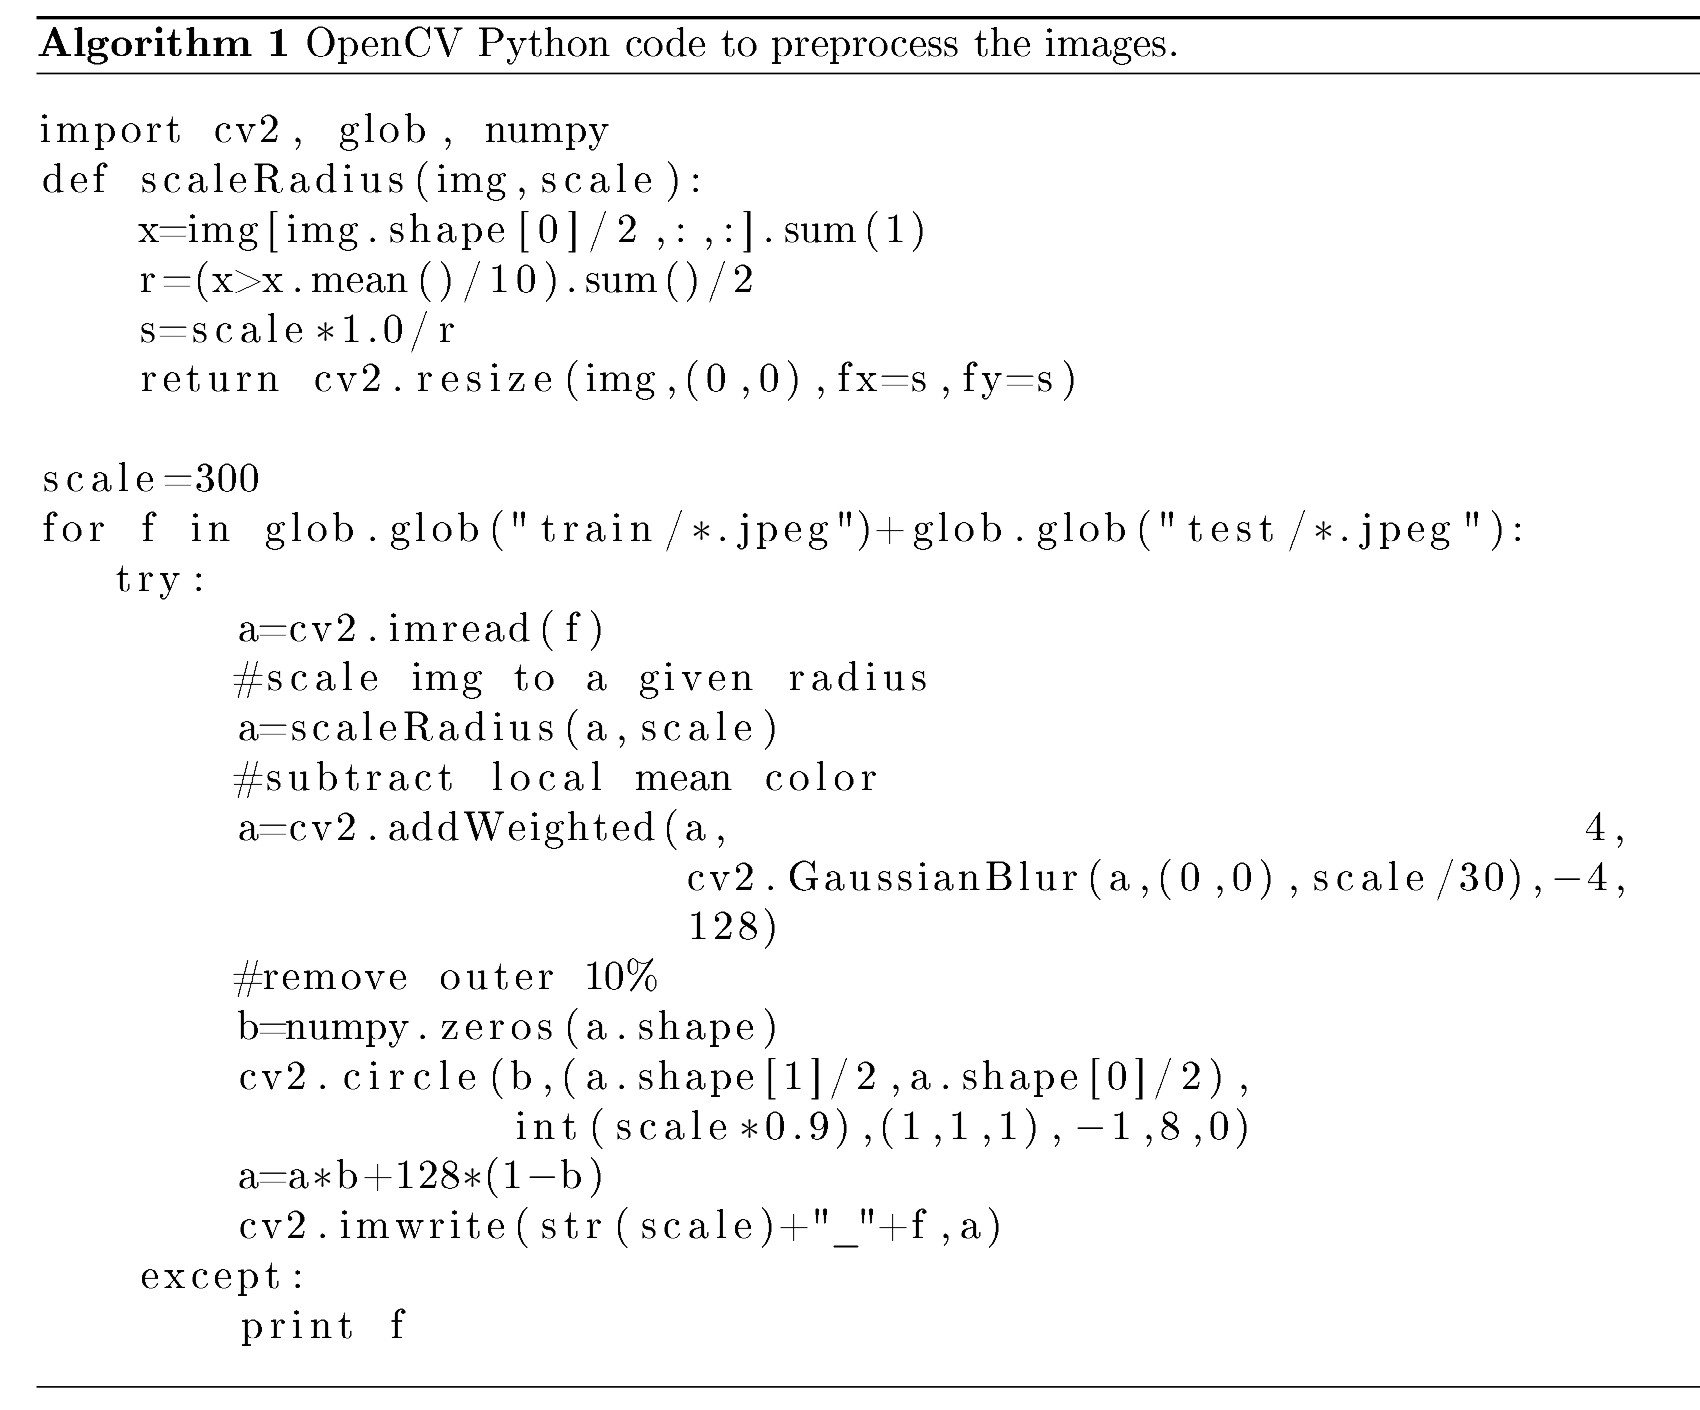
\includegraphics[width=1\textwidth]{imágenes/metodología/algoritmo_braham.jpg}
\caption*{\textit{Fuente: Adaptado de Graham (2015)}}
\end{figure}

Inicialmente las imágenes se redimensionaron para estandarizar el radio del área de 
interés en 300 o 500 píxeles, según el caso. Este paso no solo normaliza la escala entre 
muestras, sino que también optimiza el uso de recursos computacionales en etapas 
posteriores. A continuación se aplicó una normalización del color mediante la sustracción 
del promedio local de intensidad —calculado con un filtro gaussiano— y su remapeo a un 
nivel de gris medio (50\%). Esta corrección mitiga las variaciones de brillo y contraste, 
frecuentes en entornos clínicos reales.

Matemáticamente, la normalización de color se expresa como:

\begin{equation}
I_{norm}(x,y) = \frac{I(x,y) - I_{local\_mean}(x,y)}{\sigma_{local}(x,y) + \epsilon} 
\cdot k + 128
\end{equation}

donde $I(x,y)$ es la intensidad del píxel original, $I_{local\_mean}(x,y)$ es la media 
local calculada con filtro gaussiano, $\sigma_{local}(x,y)$ es la desviación estándar 
local, $\epsilon$ es una constante pequeña para evitar división por cero, y $k$ es un 
factor de escalado.

Por último se enmascaró el 10\% periférico de cada imagen mediante una máscara circular, 
eliminando así artefactos y regiones no informativas mientras se enfoca el análisis en la 
zona central de la retina. De este modo, el algoritmo garantiza que las imágenes 
procesadas presentan una mayor consistencia, lo cual resulta fundamental para etapas 
posteriores de análisis y entrenamiento de modelos. La 
Figura~\ref{fig:preprocesamiento-ejemplo} muestra la implementación paso a paso del 
procedimiento, donde se observa el escalado, la normalización del color y el recorte 
aplicados a cada imagen.

\begin{figure}[H]
	\centering
	\caption{Ejemplo visual del proceso de preprocesamiento aplicado a una imagen de 
fondo de ojo}
	\label{fig:preprocesamiento-ejemplo}
	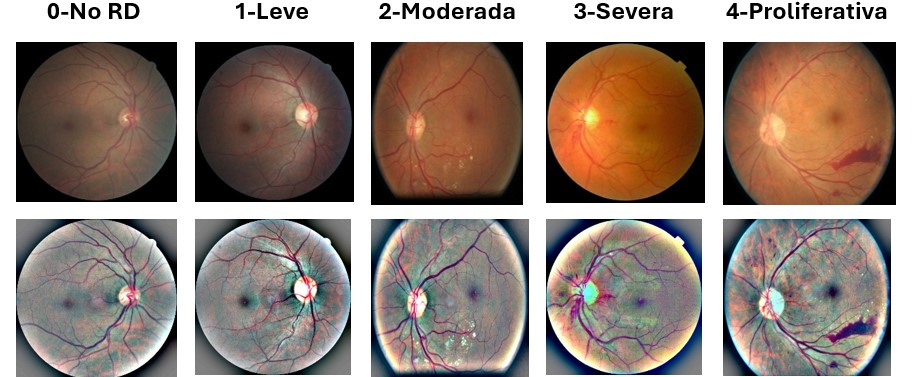
\includegraphics[width=1\textwidth]{imágenes/metodología/preprocesamiento.jpg}
	\caption*{\textit{Fuente: Elaboración propia}}
\end{figure}

\section{TECNOLOGÍAS EMPLEADAS EN EL DESARROLLO}

\subsection{Lenguaje de programación}

En el desarrollo de este trabajo de investigación, se consideraron algunos lenguajes de 
programación para la implementación de las CNNs, cada uno con aspectos particulares en el 
ámbito del procesamiento de imágenes y el aprendizaje profundo. En primer lugar se tomó 
en cuenta R, un lenguaje con una gran variedad de paquetes especializados en modelos 
estadísticos y aprendizaje automático. Sin embargo, su desempeño en tareas de deep 
learning es limitado en comparación con otros lenguajes.

Se consideró también C++, un lenguaje altamente eficiente y optimizado, utilizado en 
aplicaciones donde el rendimiento es crítico. No obstante, su curva de aprendizaje es más 
pronunciada y el desarrollo de modelos de aprendizaje profundo en este lenguaje requiere 
una mayor cantidad de código en comparación con lenguajes de alto nivel.

De este modo, se optó por Python debido a su sintaxis clara y legible que facilita la 
implementación de modelos complejos. Además, cuenta con una amplia comunidad de 
desarrolladores y científicos que contribuyen con documentación, foros de discusión y 
soluciones a problemas frecuentes, lo que resulta en un entorno de desarrollo altamente 
colaborativo. Python cuenta con un ecosistema robusto de herramientas, incluyendo 
librerías como NumPy, Pandas y Matplotlib, que son fundamentales para la manipulación y 
análisis de datos, así como para la visualización de resultados. Asimismo, su 
compatibilidad con aceleradores de hardware, como GPUs y TPUs, permite el entrenamiento 
eficiente de modelos a gran escala, reduciendo significativamente el tiempo de cómputo 
requerido.

\subsection{Entorno de desarrollo integrado (IDE)}

Se evaluaron distintos entornos de desarrollo integrados (IDE), donde cada uno ofrece 
ventajas y características específicas que pueden influir en la ejecución de los modelos. 
Uno de ellos es Jupyter Notebook, una herramienta ampliamente utilizada en investigación 
y desarrollo de proyectos de ciencia de datos debido a su flexibilidad y capacidad para 
ejecutar código de manera interactiva. Sin embargo, su uso requiere una configuración 
manual del entorno y la disponibilidad de recursos computacionales locales.

Google Colab, en cambio, es una opción muy utilizada para el desarrollo en la nube, ya 
que proporciona acceso gratuito a GPUs/TPUs y facilita la colaboración en tiempo real. No 
obstante, presenta ciertas limitaciones en cuanto a la estabilidad de las sesiones; 
acceder a una de sus GPUs gratuitas es difícil debido a la alta demanda, y el entorno se 
desconecta con frecuencia, lo que interrumpe el flujo de trabajo.

En definitiva, se seleccionaron los notebooks en la nube de Kaggle para la implementación 
debido a su estabilidad y a la posibilidad de activar una GPU en cualquier momento, con 
un límite de uso de 30 horas semanales. Esta plataforma proporciona una GPU NVIDIA Tesla 
P100 con 16 GB de memoria, además de la opción de utilizar una NVIDIA T4 x2. Este 
hardware de alto rendimiento optimiza las tareas de aprendizaje automático, agilizando 
tanto el entrenamiento de modelos como la inferencia.

\subsection{Bibliotecas y frameworks}

Se seleccionó TensorFlow junto con su API de alto nivel Keras como framework principal. 
Esta decisión se basó principalmente en que TensorFlow cuenta con una amplia adopción en 
el ámbito clínico y de investigación biomédica, ofreciendo herramientas probadas para el 
procesamiento de imágenes médicas \myfootcite{stanescu2023tensorflow}. Su integración con 
Keras simplifica la implementación de arquitecturas complejas (p. ej., ResNet, 
EfficientNet) mientras mantiene robustez en entornos productivos.

Proporciona un rendimiento eficiente en entornos con GPUs limitadas (como las ofrecidas 
por Kaggle: Tesla P100/T4), gracias a optimizaciones integradas (XLA, Grappler). Keras 
ofrece acceso directo a modelos preentrenados en TensorFlow Hub, ajustables para 
clasificación multiclase de retinopatía. Además, su ecosistema facilita el despliegue en 
clínicas mediante TensorFlow Lite o TF Serving, crucial para una futura implementación en 
entornos hospitalarios.

La suite TensorFlow Extended incluye módulos para aumento de datos (\texttt{tf.image}) y 
preprocesamiento de imágenes médicas (normalización de histogramas, ajuste de contraste), 
esenciales para abordar variabilidad en las imágenes de fondo de ojo (iluminación, 
artefactos). Aunque PyTorch ofrece mayor flexibilidad para investigación experimental, 
requiere más desarrollo manual para estas tareas. TensorFlow/Keras
demostró mayores ventajas en este proyecto al equilibrar productividad, eficiencia 
computacional y facilidad de integración.

\subsection{Especificaciones de hardware}

La Tabla~\ref{tab:hardware-tiempos} resume las especificaciones de hardware utilizadas
para el entrenamiento de los modelos, provistas por el entorno de Kaggle:

\begin{table}[H]
\centering
\renewcommand{\arraystretch}{1.3}
\caption{Especificaciones de hardware}
\label{tab:hardware-tiempos}
\begin{tabularx}{\textwidth}{l X}
\hline
\textbf{Componente} & \textbf{Especificación} \\ \hline
GPU & NVIDIA Tesla P100 (16 GB VRAM) \\
CPU & Intel Xeon (2 cores @ 2.3 GHz) \\
RAM & 13 GB \\
Framework & TensorFlow 2.12.0, Keras 2.12.0 \\
CUDA & 11.8 \\
cuDNN & 8.6 \\ \hline
\end{tabularx}
\caption*{\textit{Fuente: Elaboración propia}}
\end{table}

Los 16 GB de memoria de video (VRAM) de la Tabla~\ref{tab:hardware-tiempos} constituyen
la principal restricción práctica considerada al definir el tamaño de lote (batch size)
utilizado durante el entrenamiento, discutido más adelante en este capítulo.

\section{CONFIGURACIÓN EXPERIMENTAL Y ENTRENAMIENTO} \label{sec:config-experimental}

El proceso de entrenamiento se estructuró en dos fases consecutivas. La primera fase se 
centró en el desarrollo de un modelo para la detección binaria de retinopatía diabética 
(RD), discriminando entre casos positivos (presencia de la enfermedad) y negativos 
(ausencia de la enfermedad). Una vez validado este modelo, se procedió a una segunda fase 
de adaptación para clasificación multiclase, orientada a la categorización de la RD en 
los cinco niveles de gravedad definidos por los estándares clínicos (0: sin RD, 1: leve, 
2: moderada, 3: severa, 4: proliferativa). Esta transición responde a la necesidad de 
alinear el sistema de diagnóstico automático con los protocolos médicos establecidos, 
donde la gradación precisa de la enfermedad es crucial para la toma de decisiones 
terapéuticas.

\subsection{Configuración común para ambos clasificadores}

Para ambos clasificadores se mantuvo un marco experimental común en varios aspectos 
clave. Se implementaron bloques Multi-Head Attention luego de la salida del mapa de 
características de la red previamente entrenada, y capas GaussianNoise entre las capas 
densas. Además, se implementó una estrategia de regularización similar, utilizando en 
ambos casos Dropout, regularización L2 y parada temprana (early stopping).

En cuestión de hiperparámetros se mantuvo el mismo optimizador: Adam con un learning rate 
de $1 \times 10^{-4}$. Se eligió un tamaño de imagen de $224 \times 224$ píxeles, que es 
estándar para muchos modelos preentrenados, lo que permite un equilibrio entre el 
rendimiento computacional y la calidad de la información contenida en las imágenes. Por 
último, para ambos clasificadores se crearon modelos utilizando las mismas redes 
preentrenadas: ResNet50V2, InceptionV3, VGG19 y MobileNetV2.

La configuración de hiperparámetros no fue arbitraria: cada valor responde a alguno de
los siguientes criterios. El \textbf{learning rate} y la \textbf{tasa de Dropout} se
determinaron mediante una búsqueda sistemática (grid search) sobre nueve combinaciones
($1 \times 10^{-3}$, $1 \times 10^{-4}$ y $1 \times 10^{-5}$ para el learning rate;
$0.2$, $0.3$ y $0.5$ para el Dropout), entrenando y evaluando cada combinación sobre el
conjunto de validación; la combinación con mejor F1-score
($1 \times 10^{-4}$ y $0.2$, respectivamente) fue la seleccionada. La
\textbf{regularización L2} se probó experimentalmente sobre la mejor combinación
encontrada: su efecto sobre el F1-score y el AUC-ROC resultó marginal, pero se mantuvo
como regularizador adicional junto con Dropout y GaussianNoise. El \textbf{tamaño de
lote} (batch size) de 16 responde a una restricción computacional práctica, dado el uso
de GPUs Tesla P100/T4 provistas por Kaggle (Sección~\ref{sec:preprocesamiento}) en
conjunto con la arquitectura MobileNetV2 y el bloque de atención, que incrementan el
consumo de memoria por lote. La \textbf{paciencia de early stopping} (5 épocas) y la
\textbf{desviación estándar de GaussianNoise} (0.2) corresponden a valores de uso común
en la literatura de regularización de redes neuronales profundas, dentro de los rangos
habitualmente reportados para evitar tanto un entrenamiento prematuramente interrumpido
como una perturbación excesiva de las activaciones. El \textbf{número de cabezas de
atención} (4) sigue la práctica común en bloques de atención de tamaño moderado
acoplados a arquitecturas CNN, donde se busca capturar múltiples subespacios de
representación sin incrementar excesivamente el número de parámetros del modelo.

La Tabla~\ref{tab:hiperparametros} resume los hiperparámetros específicos utilizados en
cada tipo de clasificador:

\begin{table}[H]
\centering
\renewcommand{\arraystretch}{1.3}
\caption{Configuración de hiperparámetros para clasificadores binario y multiclase}
\label{tab:hiperparametros}
\begin{tabularx}{\textwidth}{l X >{\centering\arraybackslash}p{3.2cm} >{\centering\arraybackslash}p{3.2cm}}
\hline
\textbf{Hiperparámetro} & \textbf{Descripción} & \textbf{Binario} & \textbf{Multiclase}
\\ \hline
Tamaño de entrada & Dimensiones de imagen & $224 \times 224$ & $224 \times 224$ \\
Optimizador & Algoritmo de optimización & Adam & Adam \\
Learning rate & Tasa de aprendizaje & $1 \times 10^{-4}$ & $1 \times 10^{-4}$ \\
Batch size & Tamaño de lote & 16 & 16 \\
Épocas máximas & Número máximo de épocas & 50 & 50 \\
Dropout rate & Tasa de abandono & 0.2 & 0.2 \\
L2 regularization & Factor de regularización & 0.01 & 0.01 \\
GaussianNoise std & Desviación estándar del ruido & 0.2 & 0.2 \\
Early stopping patience & Paciencia para parada temprana & 5 épocas & 5 épocas \\
Función de pérdida & Función objetivo & Binary crossentropy & Sparse categorical crossentropy \\
Cabezas de atención & Número de cabezas en Multi-Head Attention & 4 & 4 \\
Capas densas & Configuración del top model & 512-256 & 256-128 \\
Activación salida & Función de activación final & Sigmoid & Softmax \\
Neuronas salida & Número de clases & 1 & 5 \\ \hline
\end{tabularx}
\caption*{\textit{Fuente: Elaboración propia}}
\end{table}

\subsection{Configuración experimental para el clasificador binario}

Para el clasificador binario, se utilizaron capas densas con 512 y 256 neuronas, 
intercaladas entre ellas. Esta configuración de top model es ampliamente utilizada en 
problemas de clasificación binaria con redes preentrenadas. Las funciones de activación 
utilizadas en estas capas fueron ReLU, mientras que la capa de salida fue una capa densa 
con una sola neurona y función de activación Sigmoid, apropiada para clasificación 
binaria.

Todas las capas convolucionales de cada red base fueron congeladas durante la fase de 
entrenamiento, permitiendo entrenar únicamente las capas densas superiores y los bloques 
de atención. Esto facilitó evaluar la capacidad de transferencia de características desde 
el dominio general de ImageNet al dominio específico de imágenes médicas, con un 
entrenamiento rápido y controlado.

\subsection{Configuración experimental para el clasificador multiclase}

Para el clasificador multiclase, se utilizaron capas densas con 256 y 128 neuronas 
intercaladas entre ellas. Este tipo de configuración de top model suele ser de los más 
utilizados en problemas similares \myfootcite{mutawa2023transfer}. Las funciones de 
activación utilizadas en estas capas fueron ReLU. La capa de salida fue una densa con 
cinco neuronas, una para cada nivel de RD, y función de activación Softmax.

Esta combinación de funciones de activación ha tenido bastante éxito, pues han demostrado 
un alto rendimiento y eficiencia. En muchos trabajos recopilatorios se puede ver que esta 
combinación de funciones de activación —ReLU para capas intermedias y Softmax para capa 
de salida— suele ser la más común y la que mejores resultados arroja 
\myfootcite{nadeem2022deep}. En una investigación de 2020 realizada por Asadi y Jiang 
\myfootcite{asadi2020approximation}, se demostró que ambas funciones de activación son 
aproximadores universales, dándole un fundamento teórico más robusto a su uso práctico.

Todas las capas convolucionales de cada red base fueron congeladas durante esta fase de 
experimentación, permitiendo entrenar únicamente las capas densas superiores. Se utilizó 
el optimizador Adam y la función de pérdida sparse categorical crossentropy, adecuada 
para clasificación multiclase con etiquetas en formato entero. El uso de esta función de 
pérdida ha demostrado ser más efectivo en tareas similares 
\myfootcite{palaniappan2023wide}.

Al concluir el entrenamiento, los modelos fueron evaluados tanto en el conjunto de 
entrenamiento como en el de validación. Se generaron métricas clave: recuperación 
(recall), puntuación F1 y exactitud (accuracy) mediante el informe de clasificación de 
scikit-learn. Los resultados se almacenaron y organizaron para su análisis comparativo. 
Además, se elaboraron gráficos que muestran la evolución de la pérdida y exactitud 
durante el entrenamiento, lo que permitió observar visualmente el rendimiento diferencial 
de cada arquitectura.

\subsection{Arquitectura completa del modelo}

La Figura~\ref{fig:arquitectura-modelo} muestra la arquitectura completa implementada, 
desde la entrada de la imagen hasta la capa de salida:

\begin{figure}[H]
\centering
\caption{Arquitectura completa del modelo propuesto con bloques de atención y 
regularización}
\label{fig:arquitectura-modelo}
\begin{center}
\shorthandoff{>}
\begin{tikzpicture}[node distance=1cm]
\node[draw, rectangle] (input) {Imagen de entrada $224 \times 224 \times 3$};
\node[draw, rectangle, below=of input] (base) {Base CNN preentrenada (congelada)};
\node[draw, rectangle, below=of base] (attention) {Multi-Head Attention (4 heads)};
\node[draw, rectangle, below=of attention] (gap) {Global Average Pooling};
\node[draw, rectangle, below=of gap] (noise1) {GaussianNoise ($\sigma=0.2$)};
\node[draw, rectangle, below=of noise1] (dense1) {Dense (512/256) + ReLU + Dropout (0.2)
+ L2};
\node[draw, rectangle, below=of dense1] (noise2) {GaussianNoise ($\sigma=0.2$)};
\node[draw, rectangle, below=of noise2] (dense2) {Dense (256/128) + ReLU + Dropout (0.2)
+ L2};
\node[draw, rectangle, below=of dense2] (output) {Dense (1/5) + Sigmoid/Softmax};

\draw[->] (input) -- (base);
\draw[->] (base) -- (attention);
\draw[->] (attention) -- (gap);
\draw[->] (gap) -- (noise1);
\draw[->] (noise1) -- (dense1);
\draw[->] (dense1) -- (noise2);
\draw[->] (noise2) -- (dense2);
\draw[->] (dense2) -- (output);
\end{tikzpicture}
\shorthandon{>}
\end{center}
\caption*{\textit{Fuente: Elaboración propia}}
\end{figure}

En la Figura~\ref{fig:arquitectura-modelo} puede observarse que el flujo de información
pasa primero por la base CNN preentrenada (congelada) y el bloque de atención, seguido de
dos capas densas intercaladas con GaussianNoise y regularización (Dropout y L2), hasta
llegar a la capa de salida, cuyo número de neuronas y función de activación (Sigmoid o
Softmax) dependen de si se trata del clasificador binario o multiclase, respectivamente.

\subsection{Reproducibilidad y disponibilidad de código}

Para garantizar la reproducibilidad de los experimentos, se fijaron las siguientes 
semillas aleatorias:

\begin{itemize}
    \item Semilla Python random: 42
    \item Semilla NumPy: 42
    \item Semilla TensorFlow: 42
\end{itemize}

Las versiones específicas de las bibliotecas utilizadas fueron:
\begin{itemize}
    \item Python: 3.10.12
    \item TensorFlow: 2.12.0
    \item Keras: 2.12.0
    \item NumPy: 1.23.5
    \item Pandas: 1.5.3
    \item OpenCV: 4.7.0
    \item scikit-learn: 1.2.2
\end{itemize}

El código fuente completo de los experimentos está disponible en el repositorio de Kaggle 
asociado al proyecto, permitiendo la replicación exacta de todos los procedimientos 
descritos.

\section{MÉTRICAS DE EVALUACIÓN} \label{sec:metricas-evaluacion}

En los estudios de clasificación médica existen diferentes métricas de desempeño
ampliamente utilizadas. La exactitud, la sensibilidad, la especificidad, la precisión y
el F1-score son algunas de ellas, y estas medidas se emplean para evaluar el rendimiento
de un método utilizado. En las fórmulas de la Tabla~\ref{tab:metricas-evaluacion}, TP
(True Positives) y FP (False Positives) representan el número de diagnósticos
verdaderos positivos y falsos positivos, respectivamente; TN (True Negatives) y FN
(False Negatives) representan el número de diagnósticos verdaderos negativos y falsos
negativos; y N es el número total de muestras.

\begin{table}[H]
\centering
\renewcommand{\arraystretch}{1.8}
\small
\caption{Métricas de evaluación utilizadas}
\label{tab:metricas-evaluacion}
\begin{tabularx}{\textwidth}{@{}l X c@{}}
\hline
\textbf{Métrica} & \textbf{Descripción} & \textbf{Fórmula} \\ \hline
Exactitud (Accuracy) & Proporción de predicciones correctas sobre el total de
muestras; poco informativa si las clases están desbalanceadas. &
$\frac{TP + TN}{N}$ \\
Sensibilidad (Recall) & Proporción de casos positivos (con RD) detectados
correctamente; crucial para minimizar casos no detectados. &
$\frac{TP}{TP + FN}$ \\
Especificidad & Proporción de casos negativos (sin RD) identificados correctamente;
reduce las derivaciones innecesarias. &
$\frac{TN}{TN + FP}$ \\
Precisión (Precision) & Proporción de predicciones positivas que realmente lo son;
evita el sobrediagnóstico. &
$\frac{TP}{TP + FP}$ \\
F1-score & Media armónica entre precisión y sensibilidad; balancea falsos positivos
y falsos negativos. &
$2 \cdot \frac{P \cdot S}{P + S}$ \\ \hline
\end{tabularx}
\caption*{\textit{Fuente: Elaboración propia}}
\end{table}

Adicionalmente, se calculó el área bajo la curva ROC (AUC-ROC), que proporciona una
medida robusta del desempeño del clasificador independiente del umbral de decisión. Un
valor de AUC cercano a 1.0 indica un excelente desempeño discriminatorio.

Aunque todas las métricas anteriores aportan información complementaria, no todas tienen
la misma relevancia para el problema clínico abordado en este trabajo. Dado que el
sistema se plantea principalmente como una herramienta de \textbf{tamizaje} —es decir,
un primer filtro que decide qué pacientes requieren remisión a evaluación oftalmológica
especializada—, la \textbf{sensibilidad se considera la métrica prioritaria}. Un falso
negativo en este contexto implica que un paciente con retinopatía diabética no sea
remitido para evaluación especializada, retrasando un diagnóstico y tratamiento
oportunos; en cambio, un falso positivo implica, en el peor de los casos, una remisión
innecesaria a un especialista, un costo considerablemente menor en términos clínicos.
Esta priorización de la sensibilidad es, además, el criterio que sustenta la elección del
umbral de decisión: en la Sección~\ref{subsec:umbral-decision} el umbral se optimiza
maximizando el F1-score (que pondera sensibilidad y precisión por igual) en lugar de
utilizar el valor por defecto de 0.5, precisamente para evitar que el modelo favorezca la
precisión a costa de dejar pasar casos reales de RD.

Para evaluar la robustez estadística de las métricas obtenidas, se aplicó la técnica de
bootstrap con 1,000 iteraciones de remuestreo, calculando intervalos de confianza del
95\% para cada métrica. Esto permite estimar la variabilidad de las medidas de desempeño
y proporciona una evaluación más rigurosa de la confiabilidad del modelo.

En este estudio, todos los parámetros de evaluación mencionados se utilizaron para
caracterizar el desempeño del sistema propuesto desde distintas perspectivas
complementarias, aunque, como se indicó, la sensibilidad se prioriza como criterio
principal de decisión dado el enfoque de tamizaje del sistema, tanto en clasificación
binaria como multiclase.
